\documentclass[1p]{elsarticle_modified}
%\bibliographystyle{elsarticle-num}

%\usepackage[colorlinks]{hyperref}
%\usepackage{abbrmath_seonhwa} %\Abb, \Ascr, \Acal ,\Abf, \Afrak
\usepackage{amsfonts}
\usepackage{amssymb}
\usepackage{amsmath}
\usepackage{amsthm}
\usepackage{scalefnt}
\usepackage{amsbsy}
\usepackage{kotex}
\usepackage{caption}
\usepackage{subfig}
\usepackage{color}
\usepackage{graphicx}
\usepackage{xcolor} %% white, black, red, green, blue, cyan, magenta, yellow
\usepackage{float}
\usepackage{setspace}
\usepackage{hyperref}

\usepackage{tikz}
\usetikzlibrary{arrows}

\usepackage{multirow}
\usepackage{array} % fixed length table
\usepackage{hhline}

%%%%%%%%%%%%%%%%%%%%%
\makeatletter
\renewcommand*\env@matrix[1][\arraystretch]{%
	\edef\arraystretch{#1}%
	\hskip -\arraycolsep
	\let\@ifnextchar\new@ifnextchar
	\array{*\c@MaxMatrixCols c}}
\makeatother %https://tex.stackexchange.com/questions/14071/how-can-i-increase-the-line-spacing-in-a-matrix
%%%%%%%%%%%%%%%

\usepackage[normalem]{ulem}

\newcommand{\msout}[1]{\ifmmode\text{\sout{\ensuremath{#1}}}\else\sout{#1}\fi}
%SOURCE: \msout is \stkout macro in https://tex.stackexchange.com/questions/20609/strikeout-in-math-mode

\newcommand{\cancel}[1]{
	\ifmmode
	{\color{red}\msout{#1}}
	\else
	{\color{red}\sout{#1}}
	\fi
}

\newcommand{\add}[1]{
	{\color{blue}\uwave{#1}}
}

\newcommand{\replace}[2]{
	\ifmmode
	{\color{red}\msout{#1}}{\color{blue}\uwave{#2}}
	\else
	{\color{red}\sout{#1}}{\color{blue}\uwave{#2}}
	\fi
}

\newcommand{\Sol}{\mathcal{S}} %segment
\newcommand{\D}{D} %diagram
\newcommand{\A}{\mathcal{A}} %arc


%%%%%%%%%%%%%%%%%%%%%%%%%%%%%5 test

\def\sl{\operatorname{\textup{SL}}(2,\Cbb)}
\def\psl{\operatorname{\textup{PSL}}(2,\Cbb)}
\def\quan{\mkern 1mu \triangleright \mkern 1mu}

\theoremstyle{definition}
\newtheorem{thm}{Theorem}[section]
\newtheorem{prop}[thm]{Proposition}
\newtheorem{lem}[thm]{Lemma}
\newtheorem{ques}[thm]{Question}
\newtheorem{cor}[thm]{Corollary}
\newtheorem{defn}[thm]{Definition}
\newtheorem{exam}[thm]{Example}
\newtheorem{rmk}[thm]{Remark}
\newtheorem{alg}[thm]{Algorithm}

\newcommand{\I}{\sqrt{-1}}
\begin{document}

%\begin{frontmatter}
%
%\title{Boundary parabolic representations of knots up to 8 crossings}
%
%%% Group authors per affiliation:
%\author{Yunhi Cho} 
%\address{Department of Mathematics, University of Seoul, Seoul, Korea}
%\ead{yhcho@uos.ac.kr}
%
%
%\author{Seonhwa Kim} %\fnref{s_kim}}
%\address{Center for Geometry and Physics, Institute for Basic Science, Pohang, 37673, Korea}
%\ead{ryeona17@ibs.re.kr}
%
%\author{Hyuk Kim}
%\address{Department of Mathematical Sciences, Seoul National University, Seoul 08826, Korea}
%\ead{hyukkim@snu.ac.kr}
%
%\author{Seokbeom Yoon}
%\address{Department of Mathematical Sciences, Seoul National University, Seoul, 08826,  Korea}
%\ead{sbyoon15@snu.ac.kr}
%
%\begin{abstract}
%We find all boundary parabolic representation of knots up to 8 crossings.
%
%\end{abstract}
%\begin{keyword}
%    \MSC[2010] 57M25 
%\end{keyword}
%
%\end{frontmatter}

%\linenumbers
%\tableofcontents
%
\newcommand\colored[1]{\textcolor{white}{\rule[-0.35ex]{0.8em}{1.4ex}}\kern-0.8em\color{red} #1}%
%\newcommand\colored[1]{\textcolor{white}{ #1}\kern-2.17ex	\textcolor{white}{ #1}\kern-1.81ex	\textcolor{white}{ #1}\kern-2.15ex\color{red}#1	}

{\Large $\underline{12n_{0062}~(K12n_{0062})}$}

\setlength{\tabcolsep}{10pt}
\renewcommand{\arraystretch}{1.6}
\vspace{1cm}\begin{tabular}{m{100pt}>{\centering\arraybackslash}m{274pt}}
\multirow{5}{120pt}{
	\centering
	\includegraphics[width=112pt]{../../../GIT/diagram.site/Diagrams/png/2151_12n_0062.png}\\
\ \ \ A knot diagram\footnotemark}&
\allowdisplaybreaks
\textbf{Linearized knot diagam} \\
\cline{2-2}
 &
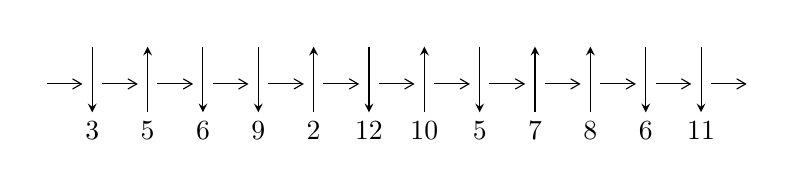
\begin{tikzpicture}[x=20pt, y=17pt]
	% nodes
	\node (C0) at (0, 0) {};
	\node (C1) at (1, 0) {};
	\node (C1U) at (1, +1) {};
	\node (C1D) at (1, -1) {3};

	\node (C2) at (2, 0) {};
	\node (C2U) at (2, +1) {};
	\node (C2D) at (2, -1) {5};

	\node (C3) at (3, 0) {};
	\node (C3U) at (3, +1) {};
	\node (C3D) at (3, -1) {6};

	\node (C4) at (4, 0) {};
	\node (C4U) at (4, +1) {};
	\node (C4D) at (4, -1) {9};

	\node (C5) at (5, 0) {};
	\node (C5U) at (5, +1) {};
	\node (C5D) at (5, -1) {2};

	\node (C6) at (6, 0) {};
	\node (C6U) at (6, +1) {};
	\node (C6D) at (6, -1) {12};

	\node (C7) at (7, 0) {};
	\node (C7U) at (7, +1) {};
	\node (C7D) at (7, -1) {10};

	\node (C8) at (8, 0) {};
	\node (C8U) at (8, +1) {};
	\node (C8D) at (8, -1) {5};

	\node (C9) at (9, 0) {};
	\node (C9U) at (9, +1) {};
	\node (C9D) at (9, -1) {7};

	\node (C10) at (10, 0) {};
	\node (C10U) at (10, +1) {};
	\node (C10D) at (10, -1) {8};

	\node (C11) at (11, 0) {};
	\node (C11U) at (11, +1) {};
	\node (C11D) at (11, -1) {6};

	\node (C12) at (12, 0) {};
	\node (C12U) at (12, +1) {};
	\node (C12D) at (12, -1) {11};
	\node (C13) at (13, 0) {};

	% arrows
	\draw[->,>={angle 60}]
	(C0) edge (C1) (C1) edge (C2) (C2) edge (C3) (C3) edge (C4) (C4) edge (C5) (C5) edge (C6) (C6) edge (C7) (C7) edge (C8) (C8) edge (C9) (C9) edge (C10) (C10) edge (C11) (C11) edge (C12) (C12) edge (C13) ;	\draw[->,>=stealth]
	(C1U) edge (C1D) (C2D) edge (C2U) (C3U) edge (C3D) (C4U) edge (C4D) (C5D) edge (C5U) (C6U) edge (C6D) (C7D) edge (C7U) (C8U) edge (C8D) (C9D) edge (C9U) (C10D) edge (C10U) (C11U) edge (C11D) (C12U) edge (C12D) ;
	\end{tikzpicture} \\
\hhline{~~} \\& 
\textbf{Solving Sequence} \\ \cline{2-2} 
 &
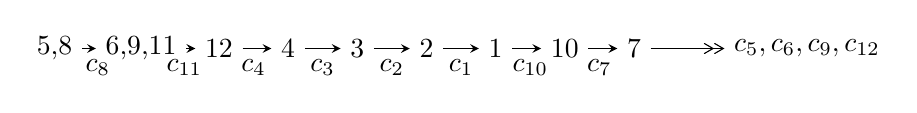
\begin{tikzpicture}[x=25pt, y=7pt]
	% node
	\node (A0) at (-1/8, 0) {5,8};
	\node (A1) at (9/8, 0) {6,9,11};
	\node (A2) at (9/4, 0) {12};
	\node (A3) at (13/4, 0) {4};
	\node (A4) at (17/4, 0) {3};
	\node (A5) at (21/4, 0) {2};
	\node (A6) at (25/4, 0) {1};
	\node (A7) at (29/4, 0) {10};
	\node (A8) at (33/4, 0) {7};
	\node (C1) at (1/2, -1) {$c_{8}$};
	\node (C2) at (7/4, -1) {$c_{11}$};
	\node (C3) at (11/4, -1) {$c_{4}$};
	\node (C4) at (15/4, -1) {$c_{3}$};
	\node (C5) at (19/4, -1) {$c_{2}$};
	\node (C6) at (23/4, -1) {$c_{1}$};
	\node (C7) at (27/4, -1) {$c_{10}$};
	\node (C8) at (31/4, -1) {$c_{7}$};
	\node (A9) at (43/4, 0) {$c_{5},c_{6},c_{9},c_{12}$};

	% edge
	\draw[->,>=stealth]	
	(A0) edge (A1) (A1) edge (A2) (A2) edge (A3) (A3) edge (A4) (A4) edge (A5) (A5) edge (A6) (A6) edge (A7) (A7) edge (A8) ;
	\draw[->>,>={angle 60}]	
	(A8) edge (A9);
\end{tikzpicture} \\ 

\end{tabular} \\

\footnotetext{
The image of knot diagram is generated by the software ``\textbf{Draw programme}" developed by Andrew Bartholomew(\url{http://www.layer8.co.uk/maths/draw/index.htm\#Running-draw}), where we modified some parts for our purpose(\url{https://github.com/CATsTAILs/LinksPainter}).
}\phantom \\ \newline 
\centering \textbf{Ideals for irreducible components\footnotemark of $X_{\text{par}}$} 
 
\begin{align*}
I^u_{1}&=\langle 
1.37658\times10^{65} u^{40}-4.47424\times10^{65} u^{39}+\cdots+1.06596\times10^{68} d+6.96533\times10^{67},\\
\phantom{I^u_{1}}&\phantom{= \langle  }1.14112\times10^{66} u^{40}-3.62494\times10^{66} u^{39}+\cdots+4.26385\times10^{68} c+2.46764\times10^{68},\\
\phantom{I^u_{1}}&\phantom{= \langle  }7.08052\times10^{74} u^{40}-1.75227\times10^{75} u^{39}+\cdots+1.49944\times10^{77} b-5.67209\times10^{77},\\
\phantom{I^u_{1}}&\phantom{= \langle  }4.57210\times10^{73} u^{40}-7.88614\times10^{75} u^{39}+\cdots+1.19955\times10^{78} a-7.69341\times10^{78},\\
\phantom{I^u_{1}}&\phantom{= \langle  }u^{41}-2 u^{40}+\cdots+512 u^2+512\rangle \\
I^u_{2}&=\langle 
- u^3 c^2+13 c^2 u^2+2 u^3 c+5 c^2 u+12 u^2 c+4 u^3+4 c^2+9 c u+24 u^2+19 d-8 c+18 u+22,\\
\phantom{I^u_{2}}&\phantom{= \langle  }-4 u^3 c^2-2 c^2 u^2+2 u^3 c+c^3-10 c^2 u+u^2 c+2 u^3-2 c^2+5 c u+2 u^2+3 c+5 u+4,\;b,\;a-1,\\
\phantom{I^u_{2}}&\phantom{= \langle  }u^4+u^3+3 u^2+2 u+1\rangle \\
\\
I^v_{1}&=\langle 
a,\;d+1,\;c+a,\;b-1,\;v^2- v+1\rangle \\
I^v_{2}&=\langle 
a,\;d,\;c-1,\;b+1,\;v^2+v+1\rangle \\
I^v_{3}&=\langle 
c,\;d+1,\;b,\;a-1,\;v-1\rangle \\
I^v_{4}&=\langle 
c,\;d+1,\;- v^2 b a+v^2 b+a v+c- v,\;b^2 v^2- b v+1\rangle \\
\end{align*}
\raggedright * 5 irreducible components of $\dim_{\mathbb{C}}=0$, with total 58 representations.\\
\raggedright * 1 irreducible components of $\dim_{\mathbb{C}}=1$ \\
\footnotetext{All coefficients of polynomials are rational numbers. But the coefficients are sometimes approximated in decimal forms when there is not enough margin.}
\newpage
\renewcommand{\arraystretch}{1}
\centering \section*{I. $I^u_{1}= \langle 1.38\times10^{65} u^{40}-4.47\times10^{65} u^{39}+\cdots+1.07\times10^{68} d+6.97\times10^{67},\;1.14\times10^{66} u^{40}-3.62\times10^{66} u^{39}+\cdots+4.26\times10^{68} c+2.47\times10^{68},\;7.08\times10^{74} u^{40}-1.75\times10^{75} u^{39}+\cdots+1.50\times10^{77} b-5.67\times10^{77},\;4.57\times10^{73} u^{40}-7.89\times10^{75} u^{39}+\cdots+1.20\times10^{78} a-7.69\times10^{78},\;u^{41}-2 u^{40}+\cdots+512 u^2+512 \rangle$}
\flushleft \textbf{(i) Arc colorings}\\
\begin{tabular}{m{7pt} m{180pt} m{7pt} m{180pt} }
\flushright $a_{5}=$&$\begin{pmatrix}0\\u\end{pmatrix}$ \\
\flushright $a_{8}=$&$\begin{pmatrix}1\\0\end{pmatrix}$ \\
\flushright $a_{6}=$&$\begin{pmatrix}-0.0000381150 u^{40}+0.00657423 u^{39}+\cdots+3.10866 u+6.41356\\-0.00472210 u^{40}+0.0116861 u^{39}+\cdots-6.53018 u+3.78280\end{pmatrix}$ \\
\flushright $a_{9}=$&$\begin{pmatrix}1\\u^2\end{pmatrix}$ \\
\flushright $a_{11}=$&$\begin{pmatrix}-0.00267627 u^{40}+0.00850156 u^{39}+\cdots+2.32863 u-0.578736\\-0.00129140 u^{40}+0.00419737 u^{39}+\cdots+1.25599 u-0.653432\end{pmatrix}$ \\
\flushright $a_{12}=$&$\begin{pmatrix}0.00393209 u^{40}-0.00559798 u^{39}+\cdots+9.49704 u-0.508301\\0.00344951 u^{40}-0.0105481 u^{39}+\cdots+5.34083 u-6.53585\end{pmatrix}$ \\
\flushright $a_{4}=$&$\begin{pmatrix}u\\u^3+u\end{pmatrix}$ \\
\flushright $a_{3}=$&$\begin{pmatrix}0.00367234 u^{40}-0.00715345 u^{39}+\cdots+6.07641 u-1.87083\\0.00428778 u^{40}-0.00271115 u^{39}+\cdots+7.55176 u+6.78311\end{pmatrix}$ \\
\flushright $a_{2}=$&$\begin{pmatrix}0.00367234 u^{40}-0.00715345 u^{39}+\cdots+6.07641 u-1.87083\\0.00169580 u^{40}+0.00233968 u^{39}+\cdots+5.67152 u+6.68520\end{pmatrix}$ \\
\flushright $a_{1}=$&$\begin{pmatrix}-0.00488842 u^{40}+0.00771683 u^{39}+\cdots-9.65835 u+0.696220\\-0.00492654 u^{40}+0.0142911 u^{39}+\cdots-6.54969 u+7.10978\end{pmatrix}$ \\
\flushright $a_{10}=$&$\begin{pmatrix}-0.00138487 u^{40}+0.00430419 u^{39}+\cdots+1.07263 u+0.0746961\\-0.00129140 u^{40}+0.00419737 u^{39}+\cdots+1.25599 u-0.653432\end{pmatrix}$ \\
\flushright $a_{7}=$&$\begin{pmatrix}-0.00138487 u^{40}+0.00430419 u^{39}+\cdots+1.07263 u+0.0746961\\0.000383620 u^{40}-0.00160154 u^{39}+\cdots-0.546942 u-0.132211\end{pmatrix}$\\&\end{tabular}
\flushleft \textbf{(ii) Obstruction class $= -1$}\\~\\
\flushleft \textbf{(iii) Cusp Shapes $= -0.00750642 u^{40}+0.0137245 u^{39}+\cdots+0.520985 u-10.6626$}\\~\\
\newpage\renewcommand{\arraystretch}{1}
\flushleft \textbf{(iv) u-Polynomials at the component}\newline \\
\begin{tabular}{m{50pt}|m{274pt}}
Crossings & \hspace{64pt}u-Polynomials at each crossing \\
\hline $$\begin{aligned}c_{1}\end{aligned}$$&$\begin{aligned}
&u^{41}+12 u^{40}+\cdots+344 u-16
\end{aligned}$\\
\hline $$\begin{aligned}c_{2},c_{5}\end{aligned}$$&$\begin{aligned}
&u^{41}+2 u^{40}+\cdots+16 u+4
\end{aligned}$\\
\hline $$\begin{aligned}c_{3}\end{aligned}$$&$\begin{aligned}
&u^{41}-2 u^{40}+\cdots+428280 u+66564
\end{aligned}$\\
\hline $$\begin{aligned}c_{4},c_{8}\end{aligned}$$&$\begin{aligned}
&u^{41}-2 u^{40}+\cdots+512 u^2+512
\end{aligned}$\\
\hline $$\begin{aligned}c_{6},c_{11}\end{aligned}$$&$\begin{aligned}
&u^{41}-8 u^{40}+\cdots-8 u+16
\end{aligned}$\\
\hline $$\begin{aligned}c_{7},c_{9},c_{10}\end{aligned}$$&$\begin{aligned}
&u^{41}+8 u^{40}+\cdots-8 u+16
\end{aligned}$\\
\hline $$\begin{aligned}c_{12}\end{aligned}$$&$\begin{aligned}
&u^{41}+10 u^{40}+\cdots+2080 u+256
\end{aligned}$\\
\hline
\end{tabular}\\~\\
\newpage\renewcommand{\arraystretch}{1}
\flushleft \textbf{(v) Riley Polynomials at the component}\newline \\
\begin{tabular}{m{50pt}|m{274pt}}
Crossings & \hspace{64pt}Riley Polynomials at each crossing \\
\hline $$\begin{aligned}c_{1}\end{aligned}$$&$\begin{aligned}
&y^{41}+36 y^{40}+\cdots+135968 y-256
\end{aligned}$\\
\hline $$\begin{aligned}c_{2},c_{5}\end{aligned}$$&$\begin{aligned}
&y^{41}+12 y^{40}+\cdots+344 y-16
\end{aligned}$\\
\hline $$\begin{aligned}c_{3}\end{aligned}$$&$\begin{aligned}
&y^{41}+60 y^{40}+\cdots+44022633912 y-4430766096
\end{aligned}$\\
\hline $$\begin{aligned}c_{4},c_{8}\end{aligned}$$&$\begin{aligned}
&y^{41}+30 y^{40}+\cdots-524288 y-262144
\end{aligned}$\\
\hline $$\begin{aligned}c_{6},c_{11}\end{aligned}$$&$\begin{aligned}
&y^{41}-10 y^{40}+\cdots+2080 y-256
\end{aligned}$\\
\hline $$\begin{aligned}c_{7},c_{9},c_{10}\end{aligned}$$&$\begin{aligned}
&y^{41}-50 y^{40}+\cdots+8224 y-256
\end{aligned}$\\
\hline $$\begin{aligned}c_{12}\end{aligned}$$&$\begin{aligned}
&y^{41}+50 y^{40}+\cdots-663040 y-65536
\end{aligned}$\\
\hline
\end{tabular}\\~\\
\newpage\flushleft \textbf{(vi) Complex Volumes and Cusp Shapes}
$$\begin{array}{c|c|c}  
\text{Solutions to }I^u_{1}& \I (\text{vol} + \sqrt{-1}CS) & \text{Cusp shape}\\
 \hline 
\begin{aligned}
u &= \phantom{-}0.280189 + 0.954581 I \\
a &= -0.857033 + 0.817841 I \\
b &= -0.265899 - 0.882324 I \\
c &= \phantom{-}0.171620 + 0.881343 I \\
d &= -0.419345 + 0.622257 I\end{aligned}
 & -1.60252 - 4.55290 I & -4.51064 + 8.08001 I \\ \hline\begin{aligned}
u &= \phantom{-}0.280189 - 0.954581 I \\
a &= -0.857033 - 0.817841 I \\
b &= -0.265899 + 0.882324 I \\
c &= \phantom{-}0.171620 - 0.881343 I \\
d &= -0.419345 - 0.622257 I\end{aligned}
 & -1.60252 + 4.55290 I & -4.51064 - 8.08001 I \\ \hline\begin{aligned}
u &= \phantom{-}0.942111 + 0.024266 I \\
a &= -0.224229 + 1.244680 I \\
b &= -0.026109 + 0.791073 I \\
c &= \phantom{-}1.54076 + 1.79047 I \\
d &= \phantom{-}0.627424 + 0.518765 I\end{aligned}
 & \phantom{-}0.87865 + 4.07350 I & -1.48942 - 7.36111 I \\ \hline\begin{aligned}
u &= \phantom{-}0.942111 - 0.024266 I \\
a &= -0.224229 - 1.244680 I \\
b &= -0.026109 - 0.791073 I \\
c &= \phantom{-}1.54076 - 1.79047 I \\
d &= \phantom{-}0.627424 - 0.518765 I\end{aligned}
 & \phantom{-}0.87865 - 4.07350 I & -1.48942 + 7.36111 I \\ \hline\begin{aligned}
u &= \phantom{-}0.100000 + 0.892301 I \\
a &= -0.052177 - 0.358577 I \\
b &= \phantom{-}0.118920 + 0.748261 I \\
c &= -0.188847 - 0.591938 I \\
d &= -0.730090 - 0.450883 I\end{aligned}
 & \phantom{-}1.46086 + 1.42227 I & \phantom{-}3.88823 - 3.83998 I \\ \hline\begin{aligned}
u &= \phantom{-}0.100000 - 0.892301 I \\
a &= -0.052177 + 0.358577 I \\
b &= \phantom{-}0.118920 - 0.748261 I \\
c &= -0.188847 + 0.591938 I \\
d &= -0.730090 + 0.450883 I\end{aligned}
 & \phantom{-}1.46086 - 1.42227 I & \phantom{-}3.88823 + 3.83998 I\\
 \hline 
 \end{array}$$\newpage$$\begin{array}{c|c|c}  
\text{Solutions to }I^u_{1}& \I (\text{vol} + \sqrt{-1}CS) & \text{Cusp shape}\\
 \hline 
\begin{aligned}
u &= \phantom{-}0.687957 + 0.421229 I \\
a &= \phantom{-}0.333750 + 0.336915 I \\
b &= \phantom{-}1.03088 + 1.01360 I \\
c &= -0.709049 - 0.230219 I \\
d &= -1.167000 - 0.190055 I\end{aligned}
 & \phantom{-}2.43397 + 0.55461 I & \phantom{-}3.61478 + 1.21885 I \\ \hline\begin{aligned}
u &= \phantom{-}0.687957 - 0.421229 I \\
a &= \phantom{-}0.333750 - 0.336915 I \\
b &= \phantom{-}1.03088 - 1.01360 I \\
c &= -0.709049 + 0.230219 I \\
d &= -1.167000 + 0.190055 I\end{aligned}
 & \phantom{-}2.43397 - 0.55461 I & \phantom{-}3.61478 - 1.21885 I \\ \hline\begin{aligned}
u &= \phantom{-}0.586118 + 0.499909 I \\
a &= -0.491451 + 0.661896 I \\
b &= -0.737846 + 0.812570 I \\
c &= \phantom{-}0.896958 + 0.907467 I \\
d &= \phantom{-}0.055470 + 0.479911 I\end{aligned}
 & -3.14860 + 0.97270 I & -10.27133 - 0.16493 I \\ \hline\begin{aligned}
u &= \phantom{-}0.586118 - 0.499909 I \\
a &= -0.491451 - 0.661896 I \\
b &= -0.737846 - 0.812570 I \\
c &= \phantom{-}0.896958 - 0.907467 I \\
d &= \phantom{-}0.055470 - 0.479911 I\end{aligned}
 & -3.14860 - 0.97270 I & -10.27133 + 0.16493 I \\ \hline\begin{aligned}
u &= -0.757570 + 0.057431 I \\
a &= \phantom{-}0.31675 + 1.45050 I \\
b &= \phantom{-}0.104479 + 0.545464 I \\
c &= \phantom{-}2.25474 + 1.86460 I \\
d &= \phantom{-}0.677009 + 0.316853 I\end{aligned}
 & \phantom{-}0.834104 - 1.057860 I & -1.84303 - 1.72199 I \\ \hline\begin{aligned}
u &= -0.757570 - 0.057431 I \\
a &= \phantom{-}0.31675 - 1.45050 I \\
b &= \phantom{-}0.104479 - 0.545464 I \\
c &= \phantom{-}2.25474 - 1.86460 I \\
d &= \phantom{-}0.677009 - 0.316853 I\end{aligned}
 & \phantom{-}0.834104 + 1.057860 I & -1.84303 + 1.72199 I\\
 \hline 
 \end{array}$$\newpage$$\begin{array}{c|c|c}  
\text{Solutions to }I^u_{1}& \I (\text{vol} + \sqrt{-1}CS) & \text{Cusp shape}\\
 \hline 
\begin{aligned}
u &= -0.748122 + 0.099272 I \\
a &= \phantom{-}0.93330 + 1.08938 I \\
b &= \phantom{-}2.35626 + 2.25935 I \\
c &= -0.756009 + 0.052947 I \\
d &= -1.208600 + 0.043942 I\end{aligned}
 & \phantom{-}0.52179 - 2.81355 I & -3.88749 + 5.15717 I \\ \hline\begin{aligned}
u &= -0.748122 - 0.099272 I \\
a &= \phantom{-}0.93330 - 1.08938 I \\
b &= \phantom{-}2.35626 - 2.25935 I \\
c &= -0.756009 - 0.052947 I \\
d &= -1.208600 - 0.043942 I\end{aligned}
 & \phantom{-}0.52179 + 2.81355 I & -3.88749 - 5.15717 I \\ \hline\begin{aligned}
u &= \phantom{-}0.004283 + 0.652626 I \\
a &= -1.55282 + 0.50485 I \\
b &= -2.68614 + 0.95227 I \\
c &= \phantom{-}0.055598 + 0.216120 I \\
d &= -0.573765 + 0.154381 I\end{aligned}
 & -0.70242 - 2.36927 I & \phantom{-}0.82941 + 4.59716 I \\ \hline\begin{aligned}
u &= \phantom{-}0.004283 - 0.652626 I \\
a &= -1.55282 - 0.50485 I \\
b &= -2.68614 - 0.95227 I \\
c &= \phantom{-}0.055598 - 0.216120 I \\
d &= -0.573765 - 0.154381 I\end{aligned}
 & -0.70242 + 2.36927 I & \phantom{-}0.82941 - 4.59716 I \\ \hline\begin{aligned}
u &= \phantom{-}0.076846 + 0.625583 I \\
a &= \phantom{-}1.20268 + 1.29382 I \\
b &= -0.275587 - 0.299772 I \\
c &= \phantom{-}0.281414 + 0.275761 I \\
d &= -0.413943 + 0.184853 I\end{aligned}
 & -0.85500 + 1.57570 I & -0.179374 + 0.776646 I \\ \hline\begin{aligned}
u &= \phantom{-}0.076846 - 0.625583 I \\
a &= \phantom{-}1.20268 - 1.29382 I \\
b &= -0.275587 + 0.299772 I \\
c &= \phantom{-}0.281414 - 0.275761 I \\
d &= -0.413943 - 0.184853 I\end{aligned}
 & -0.85500 - 1.57570 I & -0.179374 - 0.776646 I\\
 \hline 
 \end{array}$$\newpage$$\begin{array}{c|c|c}  
\text{Solutions to }I^u_{1}& \I (\text{vol} + \sqrt{-1}CS) & \text{Cusp shape}\\
 \hline 
\begin{aligned}
u &= \phantom{-}0.01326 + 1.47518 I \\
a &= -0.655430 + 0.903143 I \\
b &= \phantom{-}0.71376 - 1.96932 I \\
c &= -0.266359 - 0.027087 I \\
d &= \phantom{-}1.55037 - 0.00630 I\end{aligned}
 & \phantom{-}5.83509 - 1.34899 I & \phantom{-}0.977007 + 0.716014 I \\ \hline\begin{aligned}
u &= \phantom{-}0.01326 - 1.47518 I \\
a &= -0.655430 - 0.903143 I \\
b &= \phantom{-}0.71376 + 1.96932 I \\
c &= -0.266359 + 0.027087 I \\
d &= \phantom{-}1.55037 + 0.00630 I\end{aligned}
 & \phantom{-}5.83509 + 1.34899 I & \phantom{-}0.977007 - 0.716014 I \\ \hline\begin{aligned}
u &= -0.45410 + 1.44756 I \\
a &= \phantom{-}0.692132 + 0.807395 I \\
b &= \phantom{-}0.54174 - 2.28917 I \\
c &= -0.057340 + 0.859520 I \\
d &= \phantom{-}1.53907 + 0.21697 I\end{aligned}
 & \phantom{-}4.95290 + 7.65933 I & -2.00000 - 5.62562 I \\ \hline\begin{aligned}
u &= -0.45410 - 1.44756 I \\
a &= \phantom{-}0.692132 - 0.807395 I \\
b &= \phantom{-}0.54174 + 2.28917 I \\
c &= -0.057340 - 0.859520 I \\
d &= \phantom{-}1.53907 - 0.21697 I\end{aligned}
 & \phantom{-}4.95290 - 7.65933 I & -2.00000 + 5.62562 I \\ \hline\begin{aligned}
u &= -0.466919\phantom{ +0.000000I} \\
a &= -0.0931478\phantom{ +0.000000I} \\
b &= -0.579529\phantom{ +0.000000I} \\
c &= \phantom{-}1.52928\phantom{ +0.000000I} \\
d &= \phantom{-}0.230214\phantom{ +0.000000I}\end{aligned}
 & -1.25610\phantom{ +0.000000I} & -8.53770\phantom{ +0.000000I} \\ \hline\begin{aligned}
u &= -0.35061 + 1.53639 I \\
a &= -0.902103 + 0.091854 I \\
b &= -0.136075 + 1.212460 I \\
c &= -0.137964 - 1.319330 I \\
d &= -0.581850 - 1.030240 I\end{aligned}
 & \phantom{-}6.34261 + 3.42138 I & \phantom{-0.000000 } 0\\
 \hline 
 \end{array}$$\newpage$$\begin{array}{c|c|c}  
\text{Solutions to }I^u_{1}& \I (\text{vol} + \sqrt{-1}CS) & \text{Cusp shape}\\
 \hline 
\begin{aligned}
u &= -0.35061 - 1.53639 I \\
a &= -0.902103 - 0.091854 I \\
b &= -0.136075 - 1.212460 I \\
c &= -0.137964 + 1.319330 I \\
d &= -0.581850 + 1.030240 I\end{aligned}
 & \phantom{-}6.34261 - 3.42138 I & \phantom{-0.000000 } 0 \\ \hline\begin{aligned}
u &= \phantom{-}0.51610 + 1.49655 I \\
a &= -1.048210 - 0.118410 I \\
b &= -0.199107 - 1.232920 I \\
c &= -0.027761 + 1.384130 I \\
d &= -0.474223 + 1.062390 I\end{aligned}
 & \phantom{-}5.66064 - 9.73522 I & \phantom{-0.000000 -}0. + 7.05049 I \\ \hline\begin{aligned}
u &= \phantom{-}0.51610 - 1.49655 I \\
a &= -1.048210 + 0.118410 I \\
b &= -0.199107 + 1.232920 I \\
c &= -0.027761 - 1.384130 I \\
d &= -0.474223 - 1.062390 I\end{aligned}
 & \phantom{-}5.66064 + 9.73522 I & \phantom{-0.000000 } 0. - 7.05049 I \\ \hline\begin{aligned}
u &= \phantom{-}1.62020 + 0.13077 I \\
a &= -0.040113 - 0.941340 I \\
b &= \phantom{-}0.59368 - 2.03806 I \\
c &= -1.237690 - 0.070746 I \\
d &= -1.61926 - 0.06175 I\end{aligned}
 & \phantom{-}8.89854 + 0.19005 I & \phantom{-0.000000 } 0 \\ \hline\begin{aligned}
u &= \phantom{-}1.62020 - 0.13077 I \\
a &= -0.040113 + 0.941340 I \\
b &= \phantom{-}0.59368 + 2.03806 I \\
c &= -1.237690 + 0.070746 I \\
d &= -1.61926 + 0.06175 I\end{aligned}
 & \phantom{-}8.89854 - 0.19005 I & \phantom{-0.000000 } 0 \\ \hline\begin{aligned}
u &= -1.59450 + 0.33027 I \\
a &= -0.066671 + 1.013570 I \\
b &= \phantom{-}0.54013 + 2.15152 I \\
c &= -1.226210 + 0.179294 I \\
d &= -1.60824 + 0.15639 I\end{aligned}
 & \phantom{-}8.54414 - 6.61454 I & \phantom{-0.000000 } 0\\
 \hline 
 \end{array}$$\newpage$$\begin{array}{c|c|c}  
\text{Solutions to }I^u_{1}& \I (\text{vol} + \sqrt{-1}CS) & \text{Cusp shape}\\
 \hline 
\begin{aligned}
u &= -1.59450 - 0.33027 I \\
a &= -0.066671 - 1.013570 I \\
b &= \phantom{-}0.54013 - 2.15152 I \\
c &= -1.226210 - 0.179294 I \\
d &= -1.60824 - 0.15639 I\end{aligned}
 & \phantom{-}8.54414 + 6.61454 I & \phantom{-0.000000 } 0 \\ \hline\begin{aligned}
u &= \phantom{-}0.23388 + 1.65276 I \\
a &= -0.028955 - 0.573985 I \\
b &= \phantom{-}0.54769 + 2.08324 I \\
c &= \phantom{-}0.106730 - 0.375749 I \\
d &= \phantom{-}1.63512 - 0.11031 I\end{aligned}
 & \phantom{-}9.70458 - 3.47853 I & \phantom{-0.000000 } 0 \\ \hline\begin{aligned}
u &= \phantom{-}0.23388 - 1.65276 I \\
a &= -0.028955 + 0.573985 I \\
b &= \phantom{-}0.54769 - 2.08324 I \\
c &= \phantom{-}0.106730 + 0.375749 I \\
d &= \phantom{-}1.63512 + 0.11031 I\end{aligned}
 & \phantom{-}9.70458 + 3.47853 I & \phantom{-0.000000 } 0 \\ \hline\begin{aligned}
u &= -0.86658 + 1.51028 I \\
a &= \phantom{-}1.022730 - 0.213320 I \\
b &= \phantom{-}0.25996 - 2.32316 I \\
c &= \phantom{-}0.437465 + 1.236920 I \\
d &= \phantom{-}1.57759 + 0.41592 I\end{aligned}
 & \phantom{-}12.2320 + 15.1490 I & \phantom{-0.000000 } 0 \\ \hline\begin{aligned}
u &= -0.86658 - 1.51028 I \\
a &= \phantom{-}1.022730 + 0.213320 I \\
b &= \phantom{-}0.25996 + 2.32316 I \\
c &= \phantom{-}0.437465 - 1.236920 I \\
d &= \phantom{-}1.57759 - 0.41592 I\end{aligned}
 & \phantom{-}12.2320 - 15.1490 I & \phantom{-0.000000 } 0 \\ \hline\begin{aligned}
u &= \phantom{-}0.78943 + 1.61251 I \\
a &= \phantom{-}0.798911 + 0.089727 I \\
b &= \phantom{-}0.30028 + 2.26529 I \\
c &= \phantom{-}0.449091 - 1.082320 I \\
d &= \phantom{-}1.62479 - 0.37558 I\end{aligned}
 & \phantom{-}13.5026 - 8.6555 I & \phantom{-0.000000 } 0\\
 \hline 
 \end{array}$$\newpage$$\begin{array}{c|c|c}  
\text{Solutions to }I^u_{1}& \I (\text{vol} + \sqrt{-1}CS) & \text{Cusp shape}\\
 \hline 
\begin{aligned}
u &= \phantom{-}0.78943 - 1.61251 I \\
a &= \phantom{-}0.798911 - 0.089727 I \\
b &= \phantom{-}0.30028 - 2.26529 I \\
c &= \phantom{-}0.449091 + 1.082320 I \\
d &= \phantom{-}1.62479 + 0.37558 I\end{aligned}
 & \phantom{-}13.5026 + 8.6555 I & \phantom{-0.000000 } 0 \\ \hline\begin{aligned}
u &= \phantom{-}0.64330 + 1.72758 I \\
a &= -0.985622 - 0.148269 I \\
b &= \phantom{-}0.50633 - 1.68069 I \\
c &= \phantom{-}0.444320 - 0.855033 I \\
d &= \phantom{-}1.67606 - 0.30300 I\end{aligned}
 & \phantom{-}14.7932 - 7.9945 I & \phantom{-0.000000 } 0 \\ \hline\begin{aligned}
u &= \phantom{-}0.64330 - 1.72758 I \\
a &= -0.985622 + 0.148269 I \\
b &= \phantom{-}0.50633 + 1.68069 I \\
c &= \phantom{-}0.444320 + 0.855033 I \\
d &= \phantom{-}1.67606 + 0.30300 I\end{aligned}
 & \phantom{-}14.7932 + 7.9945 I & \phantom{-0.000000 } 0 \\ \hline\begin{aligned}
u &= -0.48873 + 1.82349 I \\
a &= -0.848856 + 0.042762 I \\
b &= \phantom{-}0.50243 + 1.74679 I \\
c &= \phantom{-}0.453903 + 0.630306 I \\
d &= \phantom{-}1.71830 + 0.22835 I\end{aligned}
 & \phantom{-}15.6167 + 1.2657 I & \phantom{-0.000000 } 0 \\ \hline\begin{aligned}
u &= -0.48873 - 1.82349 I \\
a &= -0.848856 - 0.042762 I \\
b &= \phantom{-}0.50243 - 1.74679 I \\
c &= \phantom{-}0.453903 - 0.630306 I \\
d &= \phantom{-}1.71830 - 0.22835 I\end{aligned}
 & \phantom{-}15.6167 - 1.2657 I & \phantom{-0.000000 } 0\\
 \hline 
 \end{array}$$\newpage\newpage\renewcommand{\arraystretch}{1}
\centering \section*{II. $I^u_{2}= \langle - u^3 c^2+2 u^3 c+\cdots-8 c+22,\;-4 u^3 c^2+2 u^3 c+\cdots+3 c+4,\;b,\;a-1,\;u^4+u^3+3 u^2+2 u+1 \rangle$}
\flushleft \textbf{(i) Arc colorings}\\
\begin{tabular}{m{7pt} m{180pt} m{7pt} m{180pt} }
\flushright $a_{5}=$&$\begin{pmatrix}0\\u\end{pmatrix}$ \\
\flushright $a_{8}=$&$\begin{pmatrix}1\\0\end{pmatrix}$ \\
\flushright $a_{6}=$&$\begin{pmatrix}1\\0\end{pmatrix}$ \\
\flushright $a_{9}=$&$\begin{pmatrix}1\\u^2\end{pmatrix}$ \\
\flushright $a_{11}=$&$\begin{pmatrix}c\\0.0526316 c^{2} u^{3}-0.105263 c u^{3}+\cdots+0.421053 c-1.15789\end{pmatrix}$ \\
\flushright $a_{12}=$&$\begin{pmatrix}-0.0526316 c^{2} u^{3}+0.105263 c u^{3}+\cdots+0.578947 c+1.15789\\0.0526316 c^{2} u^{3}-0.105263 c u^{3}+\cdots+0.421053 c-1.15789\end{pmatrix}$ \\
\flushright $a_{4}=$&$\begin{pmatrix}u\\u^3+u\end{pmatrix}$ \\
\flushright $a_{3}=$&$\begin{pmatrix}u^3+2 u\\u^3+u\end{pmatrix}$ \\
\flushright $a_{2}=$&$\begin{pmatrix}u^3+2 u\\u^3+u^2+2 u+1\end{pmatrix}$ \\
\flushright $a_{1}=$&$\begin{pmatrix}- u^2-1\\- u^2\end{pmatrix}$ \\
\flushright $a_{10}=$&$\begin{pmatrix}-0.0526316 c^{2} u^{3}+0.105263 c u^{3}+\cdots+0.578947 c+1.15789\\0.0526316 c^{2} u^{3}-0.105263 c u^{3}+\cdots+0.421053 c-1.15789\end{pmatrix}$ \\
\flushright $a_{7}=$&$\begin{pmatrix}-0.0526316 c^{2} u^{3}+0.105263 c u^{3}+\cdots+0.578947 c+1.15789\\-0.368421 c^{2} u^{3}-0.263158 c u^{3}+\cdots-0.947368 c+0.105263\end{pmatrix}$\\&\end{tabular}
\flushleft \textbf{(ii) Obstruction class $= -1$}\\~\\
\flushleft \textbf{(iii) Cusp Shapes $= -4 u^3-4 u^2-12 u-6$}\\~\\
\newpage\renewcommand{\arraystretch}{1}
\flushleft \textbf{(iv) u-Polynomials at the component}\newline \\
\begin{tabular}{m{50pt}|m{274pt}}
Crossings & \hspace{64pt}u-Polynomials at each crossing \\
\hline $$\begin{aligned}c_{1},c_{4},c_{8}\end{aligned}$$&$\begin{aligned}
&(u^4+u^3+3 u^2+2 u+1)^3
\end{aligned}$\\
\hline $$\begin{aligned}c_{2},c_{5}\end{aligned}$$&$\begin{aligned}
&(u^4+u^3+u^2+1)^3
\end{aligned}$\\
\hline $$\begin{aligned}c_{3}\end{aligned}$$&$\begin{aligned}
&(u^4- u^3+5 u^2+u+2)^3
\end{aligned}$\\
\hline $$\begin{aligned}c_{6},c_{7},c_{9}\\c_{10},c_{11}\end{aligned}$$&$\begin{aligned}
&u^{12}-4 u^{10}+\cdots-2 u+1
\end{aligned}$\\
\hline $$\begin{aligned}c_{12}\end{aligned}$$&$\begin{aligned}
&u^{12}+8 u^{11}+\cdots-10 u+1
\end{aligned}$\\
\hline
\end{tabular}\\~\\
\newpage\renewcommand{\arraystretch}{1}
\flushleft \textbf{(v) Riley Polynomials at the component}\newline \\
\begin{tabular}{m{50pt}|m{274pt}}
Crossings & \hspace{64pt}Riley Polynomials at each crossing \\
\hline $$\begin{aligned}c_{1},c_{4},c_{8}\end{aligned}$$&$\begin{aligned}
&(y^4+5 y^3+7 y^2+2 y+1)^3
\end{aligned}$\\
\hline $$\begin{aligned}c_{2},c_{5}\end{aligned}$$&$\begin{aligned}
&(y^4+y^3+3 y^2+2 y+1)^3
\end{aligned}$\\
\hline $$\begin{aligned}c_{3}\end{aligned}$$&$\begin{aligned}
&(y^4+9 y^3+31 y^2+19 y+4)^3
\end{aligned}$\\
\hline $$\begin{aligned}c_{6},c_{7},c_{9}\\c_{10},c_{11}\end{aligned}$$&$\begin{aligned}
&y^{12}-8 y^{11}+\cdots+10 y+1
\end{aligned}$\\
\hline $$\begin{aligned}c_{12}\end{aligned}$$&$\begin{aligned}
&y^{12}-8 y^{11}+\cdots-78 y+1
\end{aligned}$\\
\hline
\end{tabular}\\~\\
\newpage\flushleft \textbf{(vi) Complex Volumes and Cusp Shapes}
$$\begin{array}{c|c|c}  
\text{Solutions to }I^u_{2}& \I (\text{vol} + \sqrt{-1}CS) & \text{Cusp shape}\\
 \hline 
\begin{aligned}
u &= -0.395123 + 0.506844 I \\
a &= \phantom{-}1.00000\phantom{ +0.000000I} \\
b &= \phantom{-0.000000 } 0 \\
c &= \phantom{-}0.765020 - 0.640647 I \\
d &= -0.072869 - 0.359716 I\end{aligned}
 & -0.21101 + 1.41510 I & -1.82674 - 4.90874 I \\ \hline\begin{aligned}
u &= -0.395123 + 0.506844 I \\
a &= \phantom{-}1.00000\phantom{ +0.000000I} \\
b &= \phantom{-0.000000 } 0 \\
c &= -0.516348 + 0.247391 I \\
d &= -1.009230 + 0.198659 I\end{aligned}
 & -0.21101 + 1.41510 I & -1.82674 - 4.90874 I \\ \hline\begin{aligned}
u &= -0.395123 + 0.506844 I \\
a &= \phantom{-}1.00000\phantom{ +0.000000I} \\
b &= \phantom{-0.000000 } 0 \\
c &= -1.43015 + 5.08937 I \\
d &= \phantom{-}1.082100 + 0.161058 I\end{aligned}
 & -0.21101 + 1.41510 I & -1.82674 - 4.90874 I \\ \hline\begin{aligned}
u &= -0.395123 - 0.506844 I \\
a &= \phantom{-}1.00000\phantom{ +0.000000I} \\
b &= \phantom{-0.000000 } 0 \\
c &= \phantom{-}0.765020 + 0.640647 I \\
d &= -0.072869 + 0.359716 I\end{aligned}
 & -0.21101 - 1.41510 I & -1.82674 + 4.90874 I \\ \hline\begin{aligned}
u &= -0.395123 - 0.506844 I \\
a &= \phantom{-}1.00000\phantom{ +0.000000I} \\
b &= \phantom{-0.000000 } 0 \\
c &= -0.516348 - 0.247391 I \\
d &= -1.009230 - 0.198659 I\end{aligned}
 & -0.21101 - 1.41510 I & -1.82674 + 4.90874 I \\ \hline\begin{aligned}
u &= -0.395123 - 0.506844 I \\
a &= \phantom{-}1.00000\phantom{ +0.000000I} \\
b &= \phantom{-0.000000 } 0 \\
c &= -1.43015 - 5.08937 I \\
d &= \phantom{-}1.082100 - 0.161058 I\end{aligned}
 & -0.21101 - 1.41510 I & -1.82674 + 4.90874 I\\
 \hline 
 \end{array}$$\newpage$$\begin{array}{c|c|c}  
\text{Solutions to }I^u_{2}& \I (\text{vol} + \sqrt{-1}CS) & \text{Cusp shape}\\
 \hline 
\begin{aligned}
u &= -0.10488 + 1.55249 I \\
a &= \phantom{-}1.00000\phantom{ +0.000000I} \\
b &= \phantom{-0.000000 } 0 \\
c &= -0.423593 + 1.133540 I \\
d &= -0.856215 + 0.919282 I\end{aligned}
 & \phantom{-}6.79074 + 3.16396 I & \phantom{-}1.82674 - 2.56480 I \\ \hline\begin{aligned}
u &= -0.10488 + 1.55249 I \\
a &= \phantom{-}1.00000\phantom{ +0.000000I} \\
b &= \phantom{-0.000000 } 0 \\
c &= -0.291061 - 1.215200 I \\
d &= -0.730940 - 0.968963 I\end{aligned}
 & \phantom{-}6.79074 + 3.16396 I & \phantom{-}1.82674 - 2.56480 I \\ \hline\begin{aligned}
u &= -0.10488 + 1.55249 I \\
a &= \phantom{-}1.00000\phantom{ +0.000000I} \\
b &= \phantom{-0.000000 } 0 \\
c &= -0.103867 + 0.192761 I \\
d &= \phantom{-}1.58715 + 0.04968 I\end{aligned}
 & \phantom{-}6.79074 + 3.16396 I & \phantom{-}1.82674 - 2.56480 I \\ \hline\begin{aligned}
u &= -0.10488 - 1.55249 I \\
a &= \phantom{-}1.00000\phantom{ +0.000000I} \\
b &= \phantom{-0.000000 } 0 \\
c &= -0.423593 - 1.133540 I \\
d &= -0.856215 - 0.919282 I\end{aligned}
 & \phantom{-}6.79074 - 3.16396 I & \phantom{-}1.82674 + 2.56480 I \\ \hline\begin{aligned}
u &= -0.10488 - 1.55249 I \\
a &= \phantom{-}1.00000\phantom{ +0.000000I} \\
b &= \phantom{-0.000000 } 0 \\
c &= -0.291061 + 1.215200 I \\
d &= -0.730940 + 0.968963 I\end{aligned}
 & \phantom{-}6.79074 - 3.16396 I & \phantom{-}1.82674 + 2.56480 I \\ \hline\begin{aligned}
u &= -0.10488 - 1.55249 I \\
a &= \phantom{-}1.00000\phantom{ +0.000000I} \\
b &= \phantom{-0.000000 } 0 \\
c &= -0.103867 - 0.192761 I \\
d &= \phantom{-}1.58715 - 0.04968 I\end{aligned}
 & \phantom{-}6.79074 - 3.16396 I & \phantom{-}1.82674 + 2.56480 I\\
 \hline 
 \end{array}$$\newpage\newpage\renewcommand{\arraystretch}{1}
\centering \section*{III. $I^v_{1}= \langle a,\;d+1,\;c+a,\;b-1,\;v^2- v+1 \rangle$}
\flushleft \textbf{(i) Arc colorings}\\
\begin{tabular}{m{7pt} m{180pt} m{7pt} m{180pt} }
\flushright $a_{5}=$&$\begin{pmatrix}v\\0\end{pmatrix}$ \\
\flushright $a_{8}=$&$\begin{pmatrix}1\\0\end{pmatrix}$ \\
\flushright $a_{6}=$&$\begin{pmatrix}0\\1\end{pmatrix}$ \\
\flushright $a_{9}=$&$\begin{pmatrix}1\\0\end{pmatrix}$ \\
\flushright $a_{11}=$&$\begin{pmatrix}0\\-1\end{pmatrix}$ \\
\flushright $a_{12}=$&$\begin{pmatrix}0\\-1\end{pmatrix}$ \\
\flushright $a_{4}=$&$\begin{pmatrix}v\\0\end{pmatrix}$ \\
\flushright $a_{3}=$&$\begin{pmatrix}v\\- v\end{pmatrix}$ \\
\flushright $a_{2}=$&$\begin{pmatrix}v-1\\- v\end{pmatrix}$ \\
\flushright $a_{1}=$&$\begin{pmatrix}0\\-1\end{pmatrix}$ \\
\flushright $a_{10}=$&$\begin{pmatrix}1\\-1\end{pmatrix}$ \\
\flushright $a_{7}=$&$\begin{pmatrix}0\\1\end{pmatrix}$\\&\end{tabular}
\flushleft \textbf{(ii) Obstruction class $= 1$}\\~\\
\flushleft \textbf{(iii) Cusp Shapes $= 4 v+1$}\\~\\
\newpage\renewcommand{\arraystretch}{1}
\flushleft \textbf{(iv) u-Polynomials at the component}\newline \\
\begin{tabular}{m{50pt}|m{274pt}}
Crossings & \hspace{64pt}u-Polynomials at each crossing \\
\hline $$\begin{aligned}c_{1},c_{3},c_{5}\end{aligned}$$&$\begin{aligned}
&u^2- u+1
\end{aligned}$\\
\hline $$\begin{aligned}c_{2}\end{aligned}$$&$\begin{aligned}
&u^2+u+1
\end{aligned}$\\
\hline $$\begin{aligned}c_{4},c_{6},c_{8}\\c_{11},c_{12}\end{aligned}$$&$\begin{aligned}
&u^2
\end{aligned}$\\
\hline $$\begin{aligned}c_{7}\end{aligned}$$&$\begin{aligned}
&(u+1)^2
\end{aligned}$\\
\hline $$\begin{aligned}c_{9},c_{10}\end{aligned}$$&$\begin{aligned}
&(u-1)^2
\end{aligned}$\\
\hline
\end{tabular}\\~\\
\newpage\renewcommand{\arraystretch}{1}
\flushleft \textbf{(v) Riley Polynomials at the component}\newline \\
\begin{tabular}{m{50pt}|m{274pt}}
Crossings & \hspace{64pt}Riley Polynomials at each crossing \\
\hline $$\begin{aligned}c_{1},c_{2},c_{3}\\c_{5}\end{aligned}$$&$\begin{aligned}
&y^2+y+1
\end{aligned}$\\
\hline $$\begin{aligned}c_{4},c_{6},c_{8}\\c_{11},c_{12}\end{aligned}$$&$\begin{aligned}
&y^2
\end{aligned}$\\
\hline $$\begin{aligned}c_{7},c_{9},c_{10}\end{aligned}$$&$\begin{aligned}
&(y-1)^2
\end{aligned}$\\
\hline
\end{tabular}\\~\\
\newpage\flushleft \textbf{(vi) Complex Volumes and Cusp Shapes}
$$\begin{array}{c|c|c}  
\text{Solutions to }I^v_{1}& \I (\text{vol} + \sqrt{-1}CS) & \text{Cusp shape}\\
 \hline 
\begin{aligned}
v &= \phantom{-}0.500000 + 0.866025 I \\
a &= \phantom{-0.000000 } 0 \\
b &= \phantom{-}1.00000\phantom{ +0.000000I} \\
c &= \phantom{-0.000000 } 0 \\
d &= -1.00000\phantom{ +0.000000I}\end{aligned}
 & \phantom{-}1.64493 - 2.02988 I & \phantom{-}3.00000 + 3.46410 I \\ \hline\begin{aligned}
v &= \phantom{-}0.500000 - 0.866025 I \\
a &= \phantom{-0.000000 } 0 \\
b &= \phantom{-}1.00000\phantom{ +0.000000I} \\
c &= \phantom{-0.000000 } 0 \\
d &= -1.00000\phantom{ +0.000000I}\end{aligned}
 & \phantom{-}1.64493 + 2.02988 I & \phantom{-}3.00000 - 3.46410 I\\
 \hline 
 \end{array}$$\newpage\newpage\renewcommand{\arraystretch}{1}
\centering \section*{IV. $I^v_{2}= \langle a,\;d,\;c-1,\;b+1,\;v^2+v+1 \rangle$}
\flushleft \textbf{(i) Arc colorings}\\
\begin{tabular}{m{7pt} m{180pt} m{7pt} m{180pt} }
\flushright $a_{5}=$&$\begin{pmatrix}v\\0\end{pmatrix}$ \\
\flushright $a_{8}=$&$\begin{pmatrix}1\\0\end{pmatrix}$ \\
\flushright $a_{6}=$&$\begin{pmatrix}0\\-1\end{pmatrix}$ \\
\flushright $a_{9}=$&$\begin{pmatrix}1\\0\end{pmatrix}$ \\
\flushright $a_{11}=$&$\begin{pmatrix}1\\0\end{pmatrix}$ \\
\flushright $a_{12}=$&$\begin{pmatrix}1\\1\end{pmatrix}$ \\
\flushright $a_{4}=$&$\begin{pmatrix}v\\0\end{pmatrix}$ \\
\flushright $a_{3}=$&$\begin{pmatrix}v\\- v\end{pmatrix}$ \\
\flushright $a_{2}=$&$\begin{pmatrix}v+1\\- v\end{pmatrix}$ \\
\flushright $a_{1}=$&$\begin{pmatrix}0\\1\end{pmatrix}$ \\
\flushright $a_{10}=$&$\begin{pmatrix}1\\0\end{pmatrix}$ \\
\flushright $a_{7}=$&$\begin{pmatrix}1\\0\end{pmatrix}$\\&\end{tabular}
\flushleft \textbf{(ii) Obstruction class $= 1$}\\~\\
\flushleft \textbf{(iii) Cusp Shapes $= -4 v-11$}\\~\\
\newpage\renewcommand{\arraystretch}{1}
\flushleft \textbf{(iv) u-Polynomials at the component}\newline \\
\begin{tabular}{m{50pt}|m{274pt}}
Crossings & \hspace{64pt}u-Polynomials at each crossing \\
\hline $$\begin{aligned}c_{1},c_{3},c_{5}\end{aligned}$$&$\begin{aligned}
&u^2- u+1
\end{aligned}$\\
\hline $$\begin{aligned}c_{2}\end{aligned}$$&$\begin{aligned}
&u^2+u+1
\end{aligned}$\\
\hline $$\begin{aligned}c_{4},c_{7},c_{8}\\c_{9},c_{10}\end{aligned}$$&$\begin{aligned}
&u^2
\end{aligned}$\\
\hline $$\begin{aligned}c_{6}\end{aligned}$$&$\begin{aligned}
&(u-1)^2
\end{aligned}$\\
\hline $$\begin{aligned}c_{11},c_{12}\end{aligned}$$&$\begin{aligned}
&(u+1)^2
\end{aligned}$\\
\hline
\end{tabular}\\~\\
\newpage\renewcommand{\arraystretch}{1}
\flushleft \textbf{(v) Riley Polynomials at the component}\newline \\
\begin{tabular}{m{50pt}|m{274pt}}
Crossings & \hspace{64pt}Riley Polynomials at each crossing \\
\hline $$\begin{aligned}c_{1},c_{2},c_{3}\\c_{5}\end{aligned}$$&$\begin{aligned}
&y^2+y+1
\end{aligned}$\\
\hline $$\begin{aligned}c_{4},c_{7},c_{8}\\c_{9},c_{10}\end{aligned}$$&$\begin{aligned}
&y^2
\end{aligned}$\\
\hline $$\begin{aligned}c_{6},c_{11},c_{12}\end{aligned}$$&$\begin{aligned}
&(y-1)^2
\end{aligned}$\\
\hline
\end{tabular}\\~\\
\newpage\flushleft \textbf{(vi) Complex Volumes and Cusp Shapes}
$$\begin{array}{c|c|c}  
\text{Solutions to }I^v_{2}& \I (\text{vol} + \sqrt{-1}CS) & \text{Cusp shape}\\
 \hline 
\begin{aligned}
v &= -0.500000 + 0.866025 I \\
a &= \phantom{-0.000000 } 0 \\
b &= -1.00000\phantom{ +0.000000I} \\
c &= \phantom{-}1.00000\phantom{ +0.000000I} \\
d &= \phantom{-0.000000 } 0\end{aligned}
 & -1.64493 + 2.02988 I & -9.00000 - 3.46410 I \\ \hline\begin{aligned}
v &= -0.500000 - 0.866025 I \\
a &= \phantom{-0.000000 } 0 \\
b &= -1.00000\phantom{ +0.000000I} \\
c &= \phantom{-}1.00000\phantom{ +0.000000I} \\
d &= \phantom{-0.000000 } 0\end{aligned}
 & -1.64493 - 2.02988 I & -9.00000 + 3.46410 I\\
 \hline 
 \end{array}$$\newpage\newpage\renewcommand{\arraystretch}{1}
\centering \section*{V. $I^v_{3}= \langle c,\;d+1,\;b,\;a-1,\;v-1 \rangle$}
\flushleft \textbf{(i) Arc colorings}\\
\begin{tabular}{m{7pt} m{180pt} m{7pt} m{180pt} }
\flushright $a_{5}=$&$\begin{pmatrix}1\\0\end{pmatrix}$ \\
\flushright $a_{8}=$&$\begin{pmatrix}1\\0\end{pmatrix}$ \\
\flushright $a_{6}=$&$\begin{pmatrix}1\\0\end{pmatrix}$ \\
\flushright $a_{9}=$&$\begin{pmatrix}1\\0\end{pmatrix}$ \\
\flushright $a_{11}=$&$\begin{pmatrix}0\\-1\end{pmatrix}$ \\
\flushright $a_{12}=$&$\begin{pmatrix}1\\-1\end{pmatrix}$ \\
\flushright $a_{4}=$&$\begin{pmatrix}1\\0\end{pmatrix}$ \\
\flushright $a_{3}=$&$\begin{pmatrix}1\\0\end{pmatrix}$ \\
\flushright $a_{2}=$&$\begin{pmatrix}1\\0\end{pmatrix}$ \\
\flushright $a_{1}=$&$\begin{pmatrix}1\\0\end{pmatrix}$ \\
\flushright $a_{10}=$&$\begin{pmatrix}1\\-1\end{pmatrix}$ \\
\flushright $a_{7}=$&$\begin{pmatrix}0\\1\end{pmatrix}$\\&\end{tabular}
\flushleft \textbf{(ii) Obstruction class $= 1$}\\~\\
\flushleft \textbf{(iii) Cusp Shapes $= 0$}\\~\\
\newpage\renewcommand{\arraystretch}{1}
\flushleft \textbf{(iv) u-Polynomials at the component}\newline \\
\begin{tabular}{m{50pt}|m{274pt}}
Crossings & \hspace{64pt}u-Polynomials at each crossing \\
\hline $$\begin{aligned}c_{1},c_{2},c_{3}\\c_{4},c_{5},c_{8}\end{aligned}$$&$\begin{aligned}
&u
\end{aligned}$\\
\hline $$\begin{aligned}c_{6},c_{7},c_{12}\end{aligned}$$&$\begin{aligned}
&u+1
\end{aligned}$\\
\hline $$\begin{aligned}c_{9},c_{10},c_{11}\end{aligned}$$&$\begin{aligned}
&u-1
\end{aligned}$\\
\hline
\end{tabular}\\~\\
\newpage\renewcommand{\arraystretch}{1}
\flushleft \textbf{(v) Riley Polynomials at the component}\newline \\
\begin{tabular}{m{50pt}|m{274pt}}
Crossings & \hspace{64pt}Riley Polynomials at each crossing \\
\hline $$\begin{aligned}c_{1},c_{2},c_{3}\\c_{4},c_{5},c_{8}\end{aligned}$$&$\begin{aligned}
&y
\end{aligned}$\\
\hline $$\begin{aligned}c_{6},c_{7},c_{9}\\c_{10},c_{11},c_{12}\end{aligned}$$&$\begin{aligned}
&y-1
\end{aligned}$\\
\hline
\end{tabular}\\~\\
\newpage\flushleft \textbf{(vi) Complex Volumes and Cusp Shapes}
$$\begin{array}{c|c|c}  
\text{Solutions to }I^v_{3}& \I (\text{vol} + \sqrt{-1}CS) & \text{Cusp shape}\\
 \hline 
\begin{aligned}
v &= \phantom{-}1.00000\phantom{ +0.000000I} \\
a &= \phantom{-}1.00000\phantom{ +0.000000I} \\
b &= \phantom{-0.000000 } 0 \\
c &= \phantom{-0.000000 } 0 \\
d &= -1.00000\phantom{ +0.000000I}\end{aligned}
 & \phantom{-0.000000 } 0 & \phantom{-0.000000 } 0\\
 \hline 
 \end{array}$$\newpage\newpage\renewcommand{\arraystretch}{1}
\centering \section*{VI. $I^v_{4}= \langle c,\;d+1,\;- v^2 b a+v^2 b+a v+c- v,\;b^2 v^2- b v+1 \rangle$}
\flushleft \textbf{(i) Arc colorings}\\
\begin{tabular}{m{7pt} m{180pt} m{7pt} m{180pt} }
\flushright $a_{5}=$&$\begin{pmatrix}v\\0\end{pmatrix}$ \\
\flushright $a_{8}=$&$\begin{pmatrix}1\\0\end{pmatrix}$ \\
\flushright $a_{6}=$&$\begin{pmatrix}1\\b\end{pmatrix}$ \\
\flushright $a_{9}=$&$\begin{pmatrix}1\\0\end{pmatrix}$ \\
\flushright $a_{11}=$&$\begin{pmatrix}0\\-1\end{pmatrix}$ \\
\flushright $a_{12}=$&$\begin{pmatrix}1\\b-1\end{pmatrix}$ \\
\flushright $a_{4}=$&$\begin{pmatrix}v\\0\end{pmatrix}$ \\
\flushright $a_{3}=$&$\begin{pmatrix}- b v+v\\- b^2 v\end{pmatrix}$ \\
\flushright $a_{2}=$&$\begin{pmatrix}v^2 b- b v\\- b^2 v\end{pmatrix}$ \\
\flushright $a_{1}=$&$\begin{pmatrix}-1\\- b\end{pmatrix}$ \\
\flushright $a_{10}=$&$\begin{pmatrix}1\\-1\end{pmatrix}$ \\
\flushright $a_{7}=$&$\begin{pmatrix}0\\1\end{pmatrix}$\\&\end{tabular}
\flushleft \textbf{(ii) Obstruction class $= -1$}\\~\\
\flushleft \textbf{(iii) Cusp Shapes $= - b^3 v+4 b v+v^2-4$}\\~\\
\flushleft \textbf{(iv) u-Polynomials at the component} : It cannot be defined for a positive dimension component.\\~\\
\flushleft \textbf{(v) Riley Polynomials at the component} : It cannot be defined for a positive dimension component.\\~\\
\newpage\flushleft \textbf{(iv) Complex Volumes and Cusp Shapes}
$$\begin{array}{c|c|c} 
\text{Solution to }I^v_{4}& \I (\text{vol} + \sqrt{-1}CS) & \text{Cusp shape}\\
 \hline 
\begin{aligned}
v &= \cdots \\
a &= \cdots \\
b &= \cdots \\
c &= \cdots \\
d &= \cdots\end{aligned}
 & \phantom{-0.000000 } -2.02988 I & -3.94751 + 3.47096 I\\
 \hline 
 \end{array}
$$
\newpage\renewcommand{\arraystretch}{1}
\centering \section*{ VII. u-Polynomials}
\begin{tabular}{m{50pt}|m{274pt}}
Crossings & \hspace{64pt}u-Polynomials at each crossing \\
\hline $$\begin{aligned}c_{1}\end{aligned}$$&$\begin{aligned}
&u(u^2- u+1)^2(u^4+u^3+3 u^2+2 u+1)^3\\
&\cdot(u^{41}+12 u^{40}+\cdots+344 u-16)
\end{aligned}$\\
\hline $$\begin{aligned}c_{2}\end{aligned}$$&$\begin{aligned}
&u(u^2+u+1)^2(u^4+u^3+u^2+1)^{3}(u^{41}+2 u^{40}+\cdots+16 u+4)
\end{aligned}$\\
\hline $$\begin{aligned}c_{3}\end{aligned}$$&$\begin{aligned}
&u(u^2- u+1)^2(u^4- u^3+5 u^2+u+2)^3\\
&\cdot(u^{41}-2 u^{40}+\cdots+428280 u+66564)
\end{aligned}$\\
\hline $$\begin{aligned}c_{4},c_{8}\end{aligned}$$&$\begin{aligned}
&u^5(u^4+u^3+3 u^2+2 u+1)^{3}(u^{41}-2 u^{40}+\cdots+512 u^{2}+512)
\end{aligned}$\\
\hline $$\begin{aligned}c_{5}\end{aligned}$$&$\begin{aligned}
&u(u^2- u+1)^2(u^4+u^3+u^2+1)^{3}(u^{41}+2 u^{40}+\cdots+16 u+4)
\end{aligned}$\\
\hline $$\begin{aligned}c_{6}\end{aligned}$$&$\begin{aligned}
&u^2(u-1)^2(u+1)(u^{12}-4 u^{10}+\cdots-2 u+1)(u^{41}-8 u^{40}+\cdots-8 u+16)
\end{aligned}$\\
\hline $$\begin{aligned}c_{7}\end{aligned}$$&$\begin{aligned}
&u^2(u+1)^3(u^{12}-4 u^{10}+\cdots-2 u+1)(u^{41}+8 u^{40}+\cdots-8 u+16)
\end{aligned}$\\
\hline $$\begin{aligned}c_{9},c_{10}\end{aligned}$$&$\begin{aligned}
&u^2(u-1)^3(u^{12}-4 u^{10}+\cdots-2 u+1)(u^{41}+8 u^{40}+\cdots-8 u+16)
\end{aligned}$\\
\hline $$\begin{aligned}c_{11}\end{aligned}$$&$\begin{aligned}
&u^2(u-1)(u+1)^2(u^{12}-4 u^{10}+\cdots-2 u+1)(u^{41}-8 u^{40}+\cdots-8 u+16)
\end{aligned}$\\
\hline $$\begin{aligned}c_{12}\end{aligned}$$&$\begin{aligned}
&u^2(u+1)^3(u^{12}+8 u^{11}+\cdots-10 u+1)\\
&\cdot(u^{41}+10 u^{40}+\cdots+2080 u+256)
\end{aligned}$\\
\hline
\end{tabular}\newpage\renewcommand{\arraystretch}{1}
\centering \section*{ VIII. Riley Polynomials}
\begin{tabular}{m{50pt}|m{274pt}}
Crossings & \hspace{64pt}Riley Polynomials at each crossing \\
\hline $$\begin{aligned}c_{1}\end{aligned}$$&$\begin{aligned}
&y(y^2+y+1)^2(y^4+5 y^3+7 y^2+2 y+1)^3\\
&\cdot(y^{41}+36 y^{40}+\cdots+135968 y-256)
\end{aligned}$\\
\hline $$\begin{aligned}c_{2},c_{5}\end{aligned}$$&$\begin{aligned}
&y(y^2+y+1)^2(y^4+y^3+3 y^2+2 y+1)^3\\
&\cdot(y^{41}+12 y^{40}+\cdots+344 y-16)
\end{aligned}$\\
\hline $$\begin{aligned}c_{3}\end{aligned}$$&$\begin{aligned}
&y(y^2+y+1)^2(y^4+9 y^3+31 y^2+19 y+4)^3\\
&\cdot(y^{41}+60 y^{40}+\cdots+44022633912 y-4430766096)
\end{aligned}$\\
\hline $$\begin{aligned}c_{4},c_{8}\end{aligned}$$&$\begin{aligned}
&y^5(y^4+5 y^3+\cdots+2 y+1)^{3}(y^{41}+30 y^{40}+\cdots-524288 y-262144)
\end{aligned}$\\
\hline $$\begin{aligned}c_{6},c_{11}\end{aligned}$$&$\begin{aligned}
&y^2(y-1)^3(y^{12}-8 y^{11}+\cdots+10 y+1)\\
&\cdot(y^{41}-10 y^{40}+\cdots+2080 y-256)
\end{aligned}$\\
\hline $$\begin{aligned}c_{7},c_{9},c_{10}\end{aligned}$$&$\begin{aligned}
&y^2(y-1)^3(y^{12}-8 y^{11}+\cdots+10 y+1)\\
&\cdot(y^{41}-50 y^{40}+\cdots+8224 y-256)
\end{aligned}$\\
\hline $$\begin{aligned}c_{12}\end{aligned}$$&$\begin{aligned}
&y^2(y-1)^3(y^{12}-8 y^{11}+\cdots-78 y+1)\\
&\cdot(y^{41}+50 y^{40}+\cdots-663040 y-65536)
\end{aligned}$\\
\hline
\end{tabular}
\vskip 2pc
\end{document}